\documentclass[12pt]{report}
\usepackage{fontspec}
\usepackage{fullpage}
\usepackage{hyperref}
\usepackage{array}
\usepackage{url}
\usepackage{amsmath}
\usepackage{pgfplotstable}
\usepackage{algorithm2e}
\usepackage{multirow}
\usepackage{subcaption}
\usepackage{color}
\usepackage{adjustbox}
\usepackage{tikz}
\usepackage{tikz-dependency}
\usepackage{titling}
\usepackage{pdfpages}
\usepackage[round]{natbib}
\usetikzlibrary{shapes,fit,calc,er,positioning,intersections,decorations.shapes,mindmap,trees}
\tikzset{decorate sep/.style 2 args={decorate,decoration={shape backgrounds,shape=circle,
      shape size=#1,shape sep=#2}}}

\newfontfamily\hebfont[Script=Hebrew, Scale=MatchUppercase]{FreeSans}
\newcommand{\heb}[1]{\bgroup\textdir TRT\hebfont #1\egroup}

\title{
\textbf{Universal Semantic Parsing with Neural Networks} \\
\vspace{2cm}
{\large Thesis submitted for the degree of \\
``Doctor of Philosophy''}
}
\author{
By \\
Daniel Hershcovich
\vspace{2cm}
}
\date{
Submitted to the Senate of the Hebrew University \\
February, 2019
}

\begin{document}

\maketitle
\maketitle
\clearpage
\title{}
\author{
This work was carried out under the supervision of: \\
Prof. Ari Rappoport and Dr. Omri Abend
}
\date{}
\maketitle

\section*{Acknowledgments}

\pagebreak

\section*{Abstract}

Natural language processing (NLP) is a scientific and techonological field
concerned with developing methods for performing linguistic tasks automatically.
These include classifying text into categories,
tagging it for linguistic properties (such as part-of-speech),
building graphical representations for it
and generating new text according to some constraints.
For example, \textit{machine translation} is the task of generating
text in a target language given source language text.

A major effort in NLP is dedicated to \textit{natural language understanding},
which aims to be able to comprehend text, reason about it, and act upon it
in an intelligent way.
While specific use-cases or benchmarks can be solved with relatively simple
systems, understanding human language in general
requires a hierarchical representation of meaning.
Constructing this representation from text has been the goal of an extensive
line of work in \textit{semantic parsing}.
While many semantic representation schemes have been proposed,
they share many of their basic distinctions, such as between predicates
(relations, states and events) and arguments (participants).

This thesis focuses on a particular semantic representation scheme called
\textit{Universal Conceptual Cognitive Annotation} (UCCA).
A fully automatic parser is presented, and evaluated on multiple languages
(English, French and German).


\pagebreak

\tableofcontents

\chapter{Introduction}

Semantic applications in natural language processing (e.g., machine translation)
require understanding the meaning of text.
Syntactic representations suffer from limitations, since they do not
represent semantic structure directly,
which semantic annotation schemes attempt to do.
In order to represent the full range of semantic structures exhibited by
natural language, three properties should be supported: reentrancy,
representing arguments shared between predicates (Figure~\ref{fig:graduation});
non-terminal nodes for multi-word units (Figure~\ref{fig:home});
and discontinuity of semantic units in the text (Figure~\ref{fig:gave}).
The only semantic annotation scheme that supports the combination of these criteria is UCCA
\citep{abend2013universal}.


Semantic tasks in natural language processing, such as machine translation and
sentiment analysis, require understanding the meaning of text. Since text is
merely a sequence of words, it has to be represented in a way that will convey
its meaning. One simple approach, known as the bag-of-words model, looks only
at which words occur in the text. This can already provide
substantial information about the meaning, but it ignores the order of words,
which clearly conveys important information as well. The n-gram model counts
sequences of words with regard to their order, incorporating at least some of
the meaning encoded in the text structure. These models and variations of them
are quite successfully applied to a variety of
tasks\cite{mikolov2013efficient}. Nevertheless, an undeniable part in the
meaning of language resides in its hierarchical structure. Syntax is a way to
model this structure formally. Using syntactic features can improve the
performance in semantic tasks\cite{vandeghinste2013parse}.

However, syntactic annotations suffer from limitations, since they do not
represent the semantic structure of text directly. Simple manipulations such as
switching from an active construction to a passive one, which nearly do not
alter the meaning of text, can yield a significantly different syntactic
structure. Moreover, the same syntactic construct can express conceptually
distinct semantic structures\cite{abend2013ucca}.

Semantic annotation schemes attempt to represent the meaning of natural
language utterances directly. An example is semantic role
labeling\cite{baker1998framenet}\cite{paass2014semantic}, which annotates
predicates and their arguments, classifying them into specific roles. As
opposed to syntactic annotation, which reflects language-specific formal
patterns, semantic annotation corresponds to a higher level of cognitive
processing, and the same framework can potentially apply to any language.
Moreover, a rich semantic annotation scheme may be better than
syntactic annotation as an input for applications that attempt to solve a
semantic task, due to their tighter relation to the meaning of the text.

While earlier work on semantic parsing has mostly concentrated on shallow semantic analysis,
focusing on semantic role labeling of verbal argument structures,
the focus has recently shifted to parsing of more elaborate representations that account
for a wider range of phenomena. 
Most closely related to my work is Broad-Coverage Semantic Dependency Parsing (SDP).
%addressed in two SemEval tasks \cite{oepen2014semeval,oepen2015semeval},
%experimenting with the Prague tectogrammatical layer \cite{sgallhp:1986,bohmova2003prague},
%and with dependencies derived from the Enju parser\footnote{See
%\url{http://kmcs.nii.ac.jp/enju/}.}, and Lingo ERG \cite{Flic:02}.
It addresses a wide range of semantic phenomena,
and supports discontinuous units and multiple parents.
However, SDP uses
bi-lexical dependencies, disallowing non-terminal nodes, and thus faces difficulties in supporting
structures that have no clear head, such as coordination \cite{Ivanova2012who}.

Semantic parsing methods can be largely partitioned into grammar-based and grammarless methods.
Within the grammar-based literature, most work relied on Combinatory Categorial Grammar (CCG)
\cite{Steedman:00}, which allows computing semantic structure compositionally from the
syntactic derivations. Notable examples include the Boxer parser \cite{bos2005towards}
and the AMR parser by \cite{artzi2015broad}.
Other examples include parsing with Hyperedge Replacement Grammars
\cite{jones2012semantics,chiang2013parsing,peng2015synchronous} and
graph grammars \cite{koller2015semantic}.
A different line of work takes a discriminative, grammarless approach,
pursuing either graph-based methods that predict the highest ranking graph
(tree or DAG) that satisfies a given set of constraints
\cite[for AMR parsing]{flanigan2014discriminative},
or a transition-based method
that builds the parse incrementally following a series of local
decisions \cite{Nivre03anefficient}.

Another line of work addresses parsing into Abstract Meaning Representations (AMRs)
\cite{flanigan2014discriminative,vanderwende2015amr,pust2015parsing,artzi2015broad}. 
While sharing much of my work's motivation,
AMR does not ground its units in the words and constituents of the text.
This complicates the parsing task, as it requires
that the alignment between words and logical symbols be automatically
(and imprecisely) detected.
\cite{wang2015transition} applied a transition-based approach to AMR parsing,
but their method involved first syntactically parsing the input, and then converting
the resulting tree into an AMR.

In order to represent the full range of semantic structures exhibited by
natural language, there are three structural properties that should be supported.
The first is \textbf{multiple parents},
representing arguments and relations (semantic units) that are shared between predicates.
For instance, in the sentence
``After graduation, John moved to Paris'', ``John'' is an argument of both ``graduation''
and ``moved'', yielding a DAG structure rather than a tree.

The second is \textbf{non-terminal nodes} for representing units
comprising more than one word.
While bi-lexical dependencies partially circumvent this requirement, by
representing complex units in terms of their headwords, they fall short
when representing units that have no clear head.
Frequent examples of such constructions include
coordination structures (e.g., ``\textit{John and Mary} went home''),
some multi-word expressions (e.g., ``The Haves and the \textit{Have Nots}''),
and prepositional phrases.
In these cases, dependency schemes often apply some annotation convention that
selects one of the sub-units
as the head, but as different head selections are needed for different purposes,
standardization problems arise \cite{Ivanova2012who}.
For example, selecting the preposition to head prepositional phrases yields better
parsing results \cite{Schwartz:12}, while the head noun can be more useful for
information extraction purposes.

Third, semantic units may be \textbf{discontinuous} in the text. For instance, in
``John \textit{gave} everything \textit{up}''
(the phrasal verb ``gave ... up'' forms a single semantic unit.
Discontinuities are also pervasive with other multi-word
expressions \cite{schneider2014discriminative}.

\begin{figure}[h]\small\centering
  \begin{subfigure}{\textwidth}\centering
  \parbox{.1\textwidth}{\caption{}\label{fig:graduation}}
  \parbox{.4\textwidth}{
  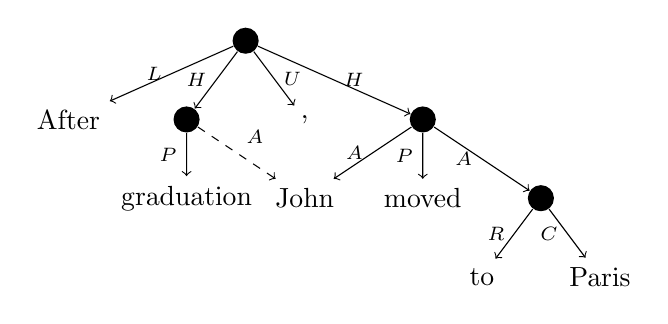
\begin{tikzpicture}[level distance=10mm, ->]
    \node (ROOT) [fill=black, circle] {}
      child {node (After) {After} edge from parent node[left] {\scriptsize $L$}}
      child {node (graduation) [fill=black, circle] {}
      {
        child {node {graduation} edge from parent node[left] {\scriptsize $P$}}
      } edge from parent node[left] {\scriptsize $H$} }
      child {node {,} edge from parent node[right] {\scriptsize $U$}}
      child {node (moved) [fill=black, circle] {}
      {
        child {node (John) {John} edge from parent node[left] {\scriptsize $A$}}
        child {node {moved} edge from parent node[left] {\scriptsize $P$}}
        child {node [fill=black, circle] {}
        {
          child {node {to} edge from parent node[left] {\scriptsize $R$}}
          child {node {Paris} edge from parent node[left] {\scriptsize $C$}}
        } edge from parent node[left] {\scriptsize $A$} }
      } edge from parent node[right] {\scriptsize $H$} }
      ;
    \draw[dashed,->] (graduation) to node [auto] {\scriptsize $A$} (John);
  \end{tikzpicture}
  }
  \end{subfigure}
  \begin{subfigure}{\textwidth}\centering
  \parbox{.1\textwidth}{\caption{}\label{fig:home}}
  \parbox{.4\textwidth}{
  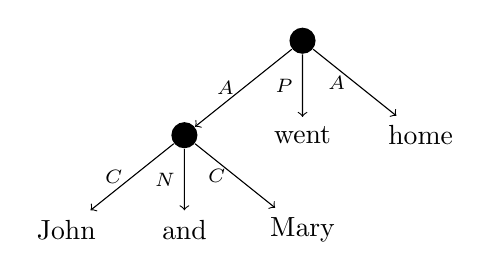
\begin{tikzpicture}[level distance=12mm, ->,
      every node/.append style={midway}]
    \node (ROOT) [fill=black, circle] {}
      child {node [fill=black, circle] {}
      {
        child {node {John} edge from parent node[left] {\scriptsize $C$}}
        child {node {and} edge from parent node[left] {\scriptsize $N$}}
        child {node {Mary} edge from parent node[left] {\scriptsize $C$}}
      } edge from parent node[left] {\scriptsize $A$} }
      child {node {went} edge from parent node[left] {\scriptsize $P$}}
      child {node {home} edge from parent node[left] {\scriptsize $A$}}
      ;
  \end{tikzpicture}
  }
  \end{subfigure}
  \begin{subfigure}{\textwidth}\centering
  \parbox{.1\textwidth}{\caption{}\label{fig:gave}}
  \parbox{.4\textwidth}{
  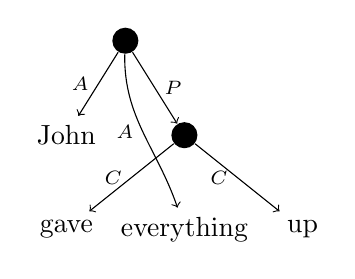
\begin{tikzpicture}[level distance=12mm, ->,
      every node/.append style={midway}]
    \node (ROOT) [fill=black, circle] {}
      child {node {John} edge from parent node[left] {\scriptsize $A$}}
      child {node [fill=black, circle] {}
      {
      	child {node {gave} edge from parent node[left] {\scriptsize $C$}}
      	child {node (everything) {everything} edge from parent[white]}
      	child {node {up} edge from parent node[left] {\scriptsize $C$}}
      } edge from parent node[right] {\scriptsize $P$} }
      ;
    \draw[bend right,->] (ROOT) to[out=-20, in=180] node [left] {\scriptsize $A$} (everything);
  \end{tikzpicture}
  }
  \end{subfigure}
  \begin{subfigure}{\textwidth}\centering
  \parbox{.1\textwidth}{\caption{}\label{fig:shower}}
  \parbox{.4\textwidth}{
  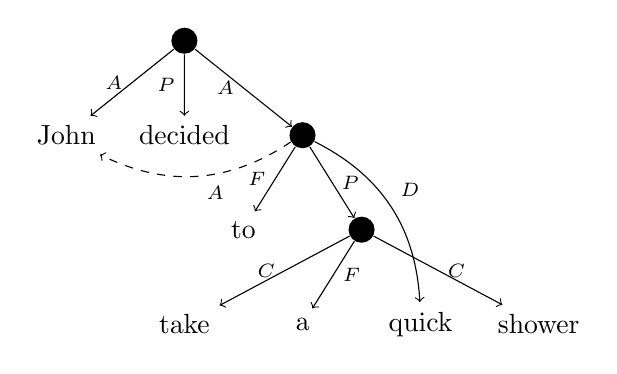
\begin{tikzpicture}[level distance=12mm, ->,
      every node/.append style={midway}]
    \node (ROOT) [fill=black, circle] {}
      child {node (John) {John} edge from parent node[left] {\scriptsize $A$}}
      child {node {decided} edge from parent node[left] {\scriptsize $P$}}
      child {node (totakeaquickshower) [fill=black, circle] {}
      {
        child {node {to} edge from parent node[left] {\scriptsize $F$}}
        child {node [fill=black, circle] {}
        {
          child {node {take} edge from parent node[left] {\scriptsize $C$}}
          child {node {a} edge from parent node[right] {\scriptsize $F$}}
          child {node (quick) {quick} edge from parent[white]}
          child {node {shower} edge from parent node[right] {\scriptsize $C$}}
        } edge from parent node[right] {\scriptsize $P$} }
      } edge from parent node[left] {\scriptsize $A$} }
      ;
    \draw[bend left,dashed,->] (totakeaquickshower) to node [auto] {\scriptsize $A$} (John);
    \draw[bend left,->] (totakeaquickshower) to node [auto] {\scriptsize $D$} (quick);
  \end{tikzpicture}
  }
  \end{subfigure}
  \caption{\label{fig:examples}
    UCCA examples.
    (\subref{fig:graduation}) includes a remote edge (dashed),
    resulting in ``John'' having two parents.
    (\subref{fig:home}) includes a coordination construction (``John and Mary'').
    (\subref{fig:gave}) includes a discontinuous unit (``gave ... up'').
    (\subref{fig:shower}) includes both a remote edge and a discontinuous unit (``take a ... shower'').
    Legend: $P$ -- Process (a Scene's main relation), $A$ -- Participant,
    $L$ -- inter-scene Linker, $H$ -- Parallel Scene, $C$ -- Center, $D$ -- Adverbial,
    $R$ -- Relator, $N$ -- Connector, $U$ -- Punctuation, $F$ -- Function unit.
  }
\end{figure}

Universal Cognitive Conceptual Annotation (UCCA)
is a cross-linguistically applicable semantic representation scheme.
It covers the predicate-argument
structures evoked by predicates of all grammatical categories, the inter-relations between them,
as well as other major linguistic phenomena.
UCCA has demonstrated applicability to multiple languages,
rapid annotation \citep{abend2017uccaapp},
stability in translation \citep{sulem2015conceptual}
and benefit for various applications
\citep{birch2016hume,choshen2018usim,sulem2018samsa,sulem2018simple}.

While semantic representation schemes are different in form and focus,
much of their semantic content is shared \citep{abend2017state}.
Recent work in semantic parsing has targeted
Abstract Meaning Representation \citep{banarescu2013abstract} and
Semantic Dependencies \citep{oepen2016towards}.
Universal Dependencies \citep{nivre2016universal}
is a \textit{syntactic} dependency scheme aiming for cross-lingual consistency,
whose annotation is often similar to the common practice in semantic treebanks
(Figure~\ref{fig:original_example_ud}).

\begin{figure}[t]
  \centering
    \begin{dependency}[text only label, label style={above,font=\tt}, font=\small]
    \begin{deptext}[column sep=.8em,ampersand replacement=\^]
    After \^ graduation \^ , \^ John \^ moved \^ to \^ Paris \\
    \end{deptext}
        \depedge[edge unit distance=1ex]{2}{1}{case}
        \depedge[edge unit distance=1ex]{2}{3}{punct}
        \depedge[edge unit distance=1ex]{5}{4}{nsubj}
        \depedge[edge unit distance=1ex, edge end x offset=-2pt]{5}{2}{obl}
        \depedge[edge unit distance=1ex]{7}{6}{case}
        \deproot[edge unit distance=1.5ex]{5}{root}
        \depedge[edge unit distance=1.5ex]{5}{7}{obl}
    \end{dependency}
\caption{Example UD tree, demonstrating practices common in semantic annotation:
linking content words to content words, and preference of lexical heads over functional ones.
\label{fig:original_example_ud}}
\end{figure}

My research is concerned with learning to parse UCCA graphs from text, representing its semantics.
I introduce a general graph parser,
and investigate the relationship with other representations to find beneficial commonalities and
differences highlighting the potential utility of semantic parsers for text understanding applications.
The analysis also exposes challenges semantic parsers must address,
and potential sources for improvement.

\subsection*{Summary of Research Goals}

In my research, I pursue the following goals:

\begin{itemize}
  \item Developing techniques for general graph parsing.
    Specifically, devising a method for automatic prediction of UCCA
    structure given plain text.
  \item Investigating and quantifying the relationship between the content
    captured in UCCA and other semantic or syntactic representations.
  \item Taking advantage of the similarities to other schemes,
    to improve UCCA parsing by learning common distinctions.
\end{itemize}

\chapter{Methodology}

\subsection*{Transition-Based Parsing}

Transition-based parsers \citep{Nivre03anefficient} build trees or graphs
as they scan the text incrementally.
The parse is created by applying a \textit{transition} at each step to the parser state,
defined using a buffer of tokens and nodes to be processed,
a stack of nodes currently being processed,
and a graph of constructed nodes and labeled edges.
A classifier is used at each step to select the next transition based on features
that encode the parser's current state.
During training, an oracle creates training instances for the classifier,
based on the gold-standard annotation.

The transition-based approach has produced some of the best
results in syntactic dependency parsing
\citep{kiperwasser2016simple,andor2016globally}, and has also demonstrated
strong performance in a variety of other semantic and syntactic settings
\citep{maier2015discontinuous,damonte-17}.
Transition-based methods are a natural starting point for UCCA parsing,
as the set of distinctions it represents is similar in spirit to the distinctions
conveyed by dependency schemes.


\subsection*{Neural Networks}

Neural networks are powerful machine learning models.
They have yielded state-of-the-art results in many fields,
including natural language processing \citep{goldberg2016primer}.
Inspired by the brain's computation mechanism,
artificial neural networks operate on dense input representations
by a combination of linear and non-linear transformations.

Language data is commonly manifested as sequences
(e.g., sentences are sequences of words).
Recurrent neural networks \citep{elman1990finding} allow representing
arbitrarily sized sequences in a fixed-size vector,
without ignoring the structured properties of the input.
A specific flavor called Long Short Term Memory
(LSTM) is very common as it learns relatively long-term dependencies.
A bidirectional recurrent neural network, such as a BiLSTM,
takes into account both the past and future.


\subsection*{Multitask Learning}

Multitask learning \citep{caruana1998multitask} allows exploiting the overlap between tasks
to effectively extend the training data, 
and has greatly advanced with neural networks and representation learning.
It has been used over the years for NLP tasks with varying degrees of similarity.

Neural multitask learning has mostly been effective in tackling formally similar
tasks \citep{P16-2038},
including
multilingual syntactic dependency parsing \citep{Q16-1031,guo2016exploiting},
as well as multilingual \citep{duong2017multilingual},
and cross-domain semantic parsing \citep{herzig-berant:2017:Short,W17-2607}.

Sharing parameters with a low-level task
has shown great benefit for transition-based syntactic parsing
\citep{bohnet2012transition,Zhang2016StackpropagationIR,constant-nivre:2016:P16-1,more2016joint}.
Recent work has achieved state-of-the-art results in multiple NLP tasks
by jointly learning the tasks forming the NLP standard pipeline using 
a single neural model \citep{collobert2011natural,D17-1206},
thereby avoiding cascading errors, common in pipelines.

\paragraph{Data.}

Experiments are performed on the English Wikipedia UCCA corpus (Wiki),
the \textit{Twenty Thousand Leagues Under the Sea} UCCA corpora (20K),
annotated in English, French and German;
LDC2017T10 for AMR;
the DM representation from SDP 2016;
and all English, French and German treebanks from UD v2.1.


\paragraph{Evaluation.}
Comparing UCCA structures
$G_p=(V_p,E_p,\ell_p)$ and $G_g=(V_g,E_g,\ell_g)$,
over the same sequence of terminals $W = \{w_1,\ldots,w_n\}$
is done as follows.
For an edge $e=(u,v)$ in either graph, its yield $y(e) \subseteq W$ is the
set of terminals in $W$ that are descendants of $v$.
Define the set of \textit{mutual edges} between $G_p$ and $G_g$:
\[
    M(G_p,G_g) =
    \left\{(e_1,e_2) \in E_p \times E_g \;|\;
    y(e_1) = y(e_2) \wedge \ell_p(e_1)=\ell_g(e_2)\right\}
\]

Labeled precision and recall are defined by dividing $|M(G_p,G_g)|$ by $|E_p|$ and $|E_g|$, respectively,
and F-score by taking their harmonic mean.
Two variants are reported: one where we consider only primary edges,
and another for remote edges


\paragraph{Settings.}

The following settings are explored:
(1) in-domain setting in English, training and testing on Wiki;
(2) out-of-domain setting in English, training on Wiki and testing on 20K;
(3) French in-domain setting, where available training dataset is small,
training and testing on 20K;
(4) German in-domain setting on 20K, with somewhat noisy annotation.
For multitask experiments, we use unlabeled AMR, DM and UD parsing as auxiliary tasks in English,
and unlabeled UD parsing in French and German.

\paragraph{Baselines.}
As no direct comparison with existing parsers is possible,
baselines are bi-lexical dependency graph parsers,
which support reentrancy and discontinuity but not non-terminal nodes;
and \textit{tree approximation}, converting UCCA to (bi-lexical) trees
and evaluating constituency and dependency tree parsers on them.
Baselines are DAGParser \citep{ribeyre-villemontedelaclergerie-seddah:2014:SemEval} and
TurboParser \citep{almeida-martins:2015:SemEval},
two bi-lexical dependency graph parsers;
\textsc{uparse} \citep{maier-lichte:2016:DiscoNLP},
a transition-based constituency parser supporting discontinuous constituents;
and two bi-lexical tree parsers:
MaltParser \citep{nivre2007maltparser},
and the stack LSTM parser \citep{dyer2015transition}.


\chapter{A Transition-Based Directed Acyclic Graph Parser for UCCA \\ (Published in ACL 2017)}

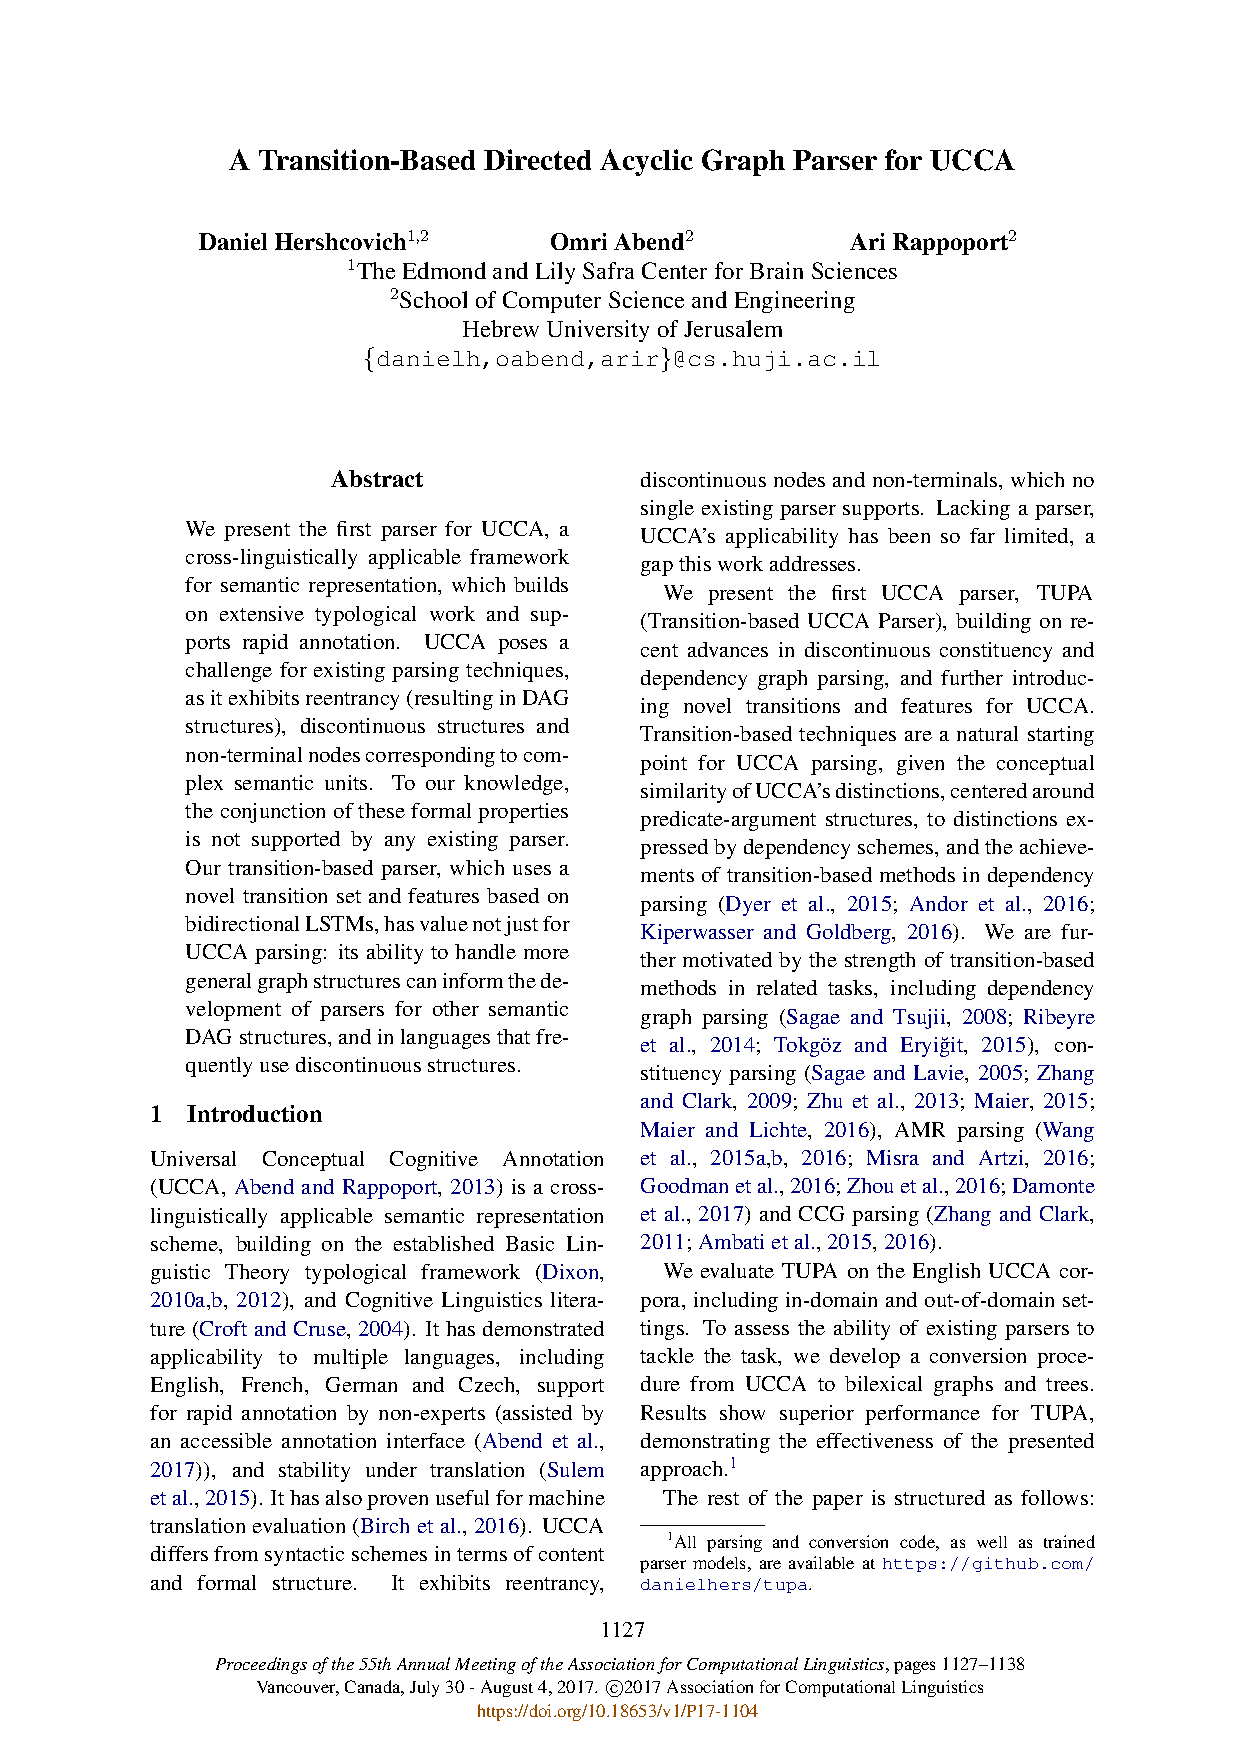
\includepdf[pages=-]{P17-1104.pdf}

\chapter{Multitask Parsing Across Semantic Representations \\ (Published in ACL 2018)}

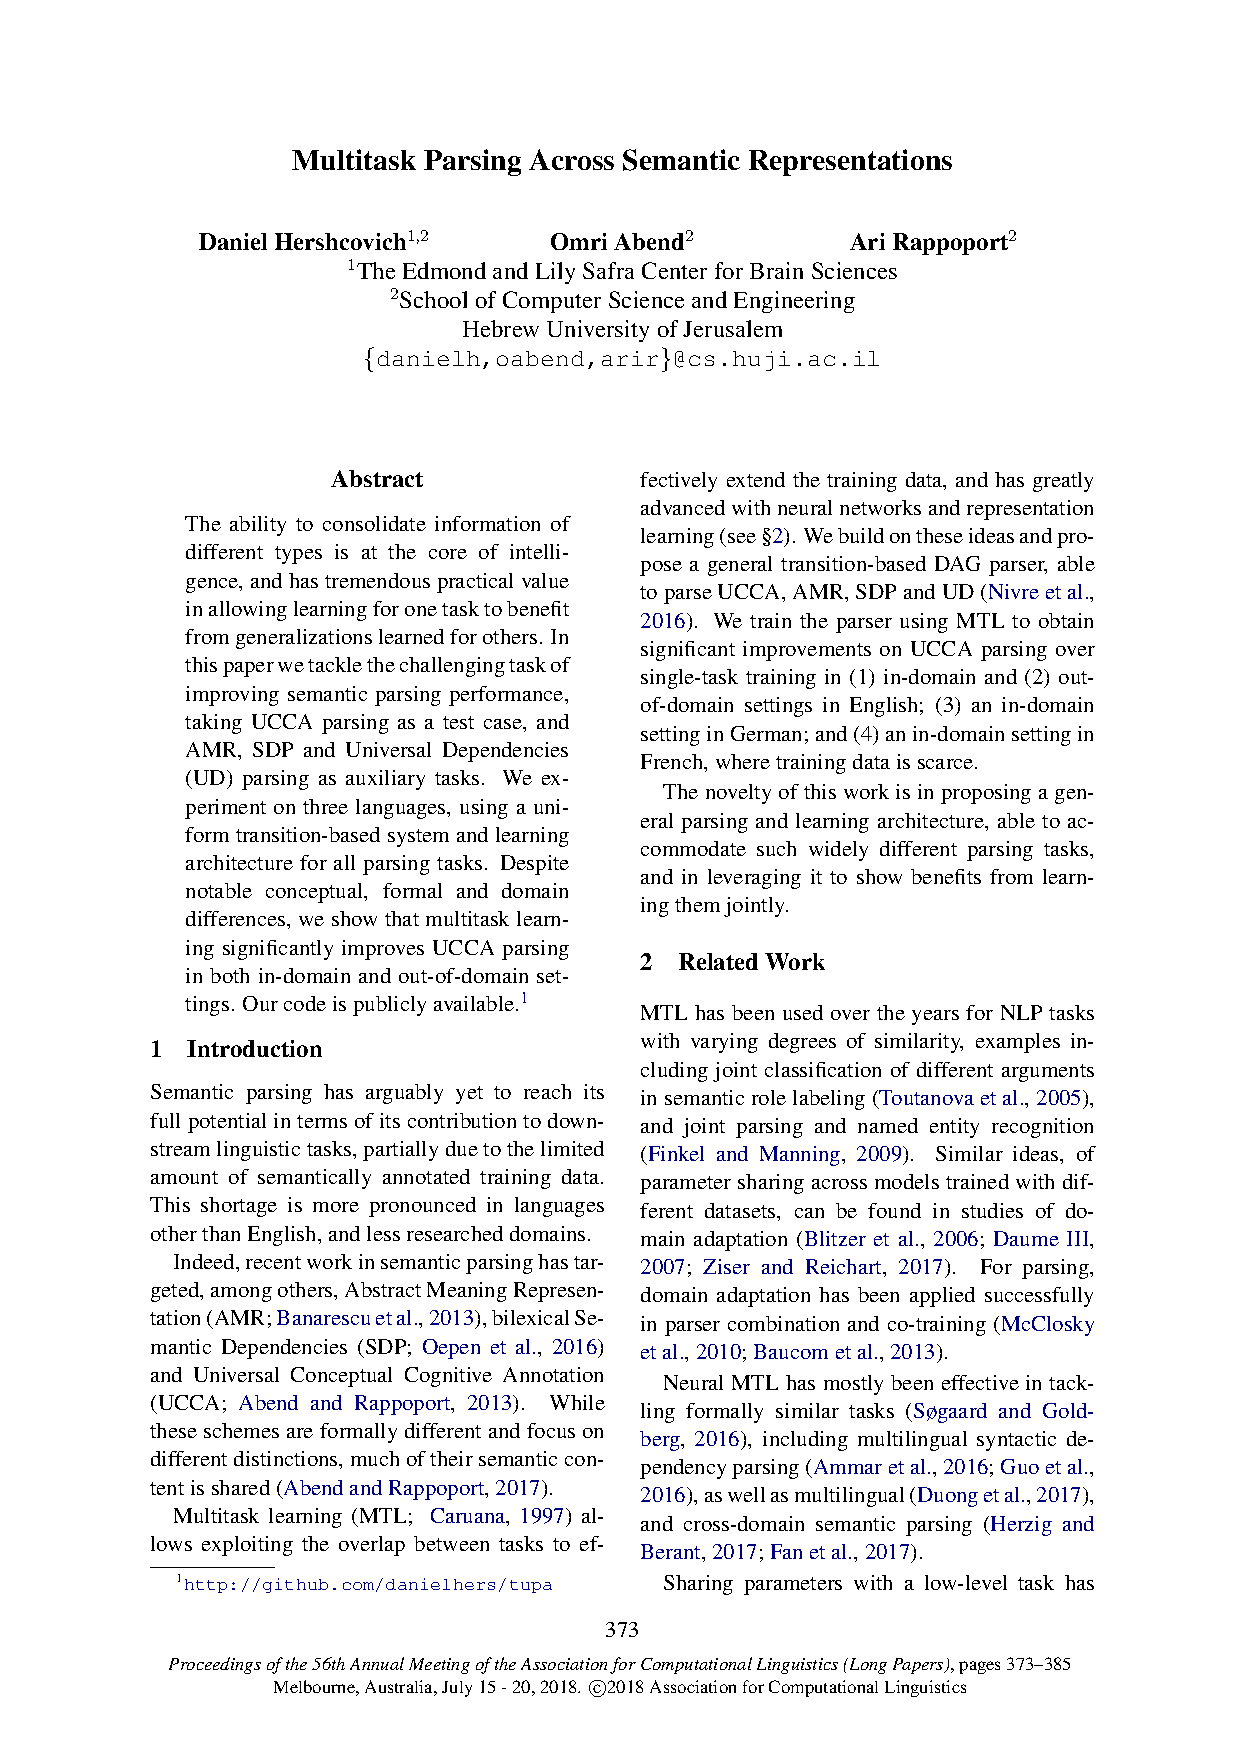
\includepdf[pages=-]{P18-1035.pdf}

\chapter{Universal Dependency Parsing with a General Transition-Based DAG Parser \\ (Published in CoNLL 2018 Shared Task)}

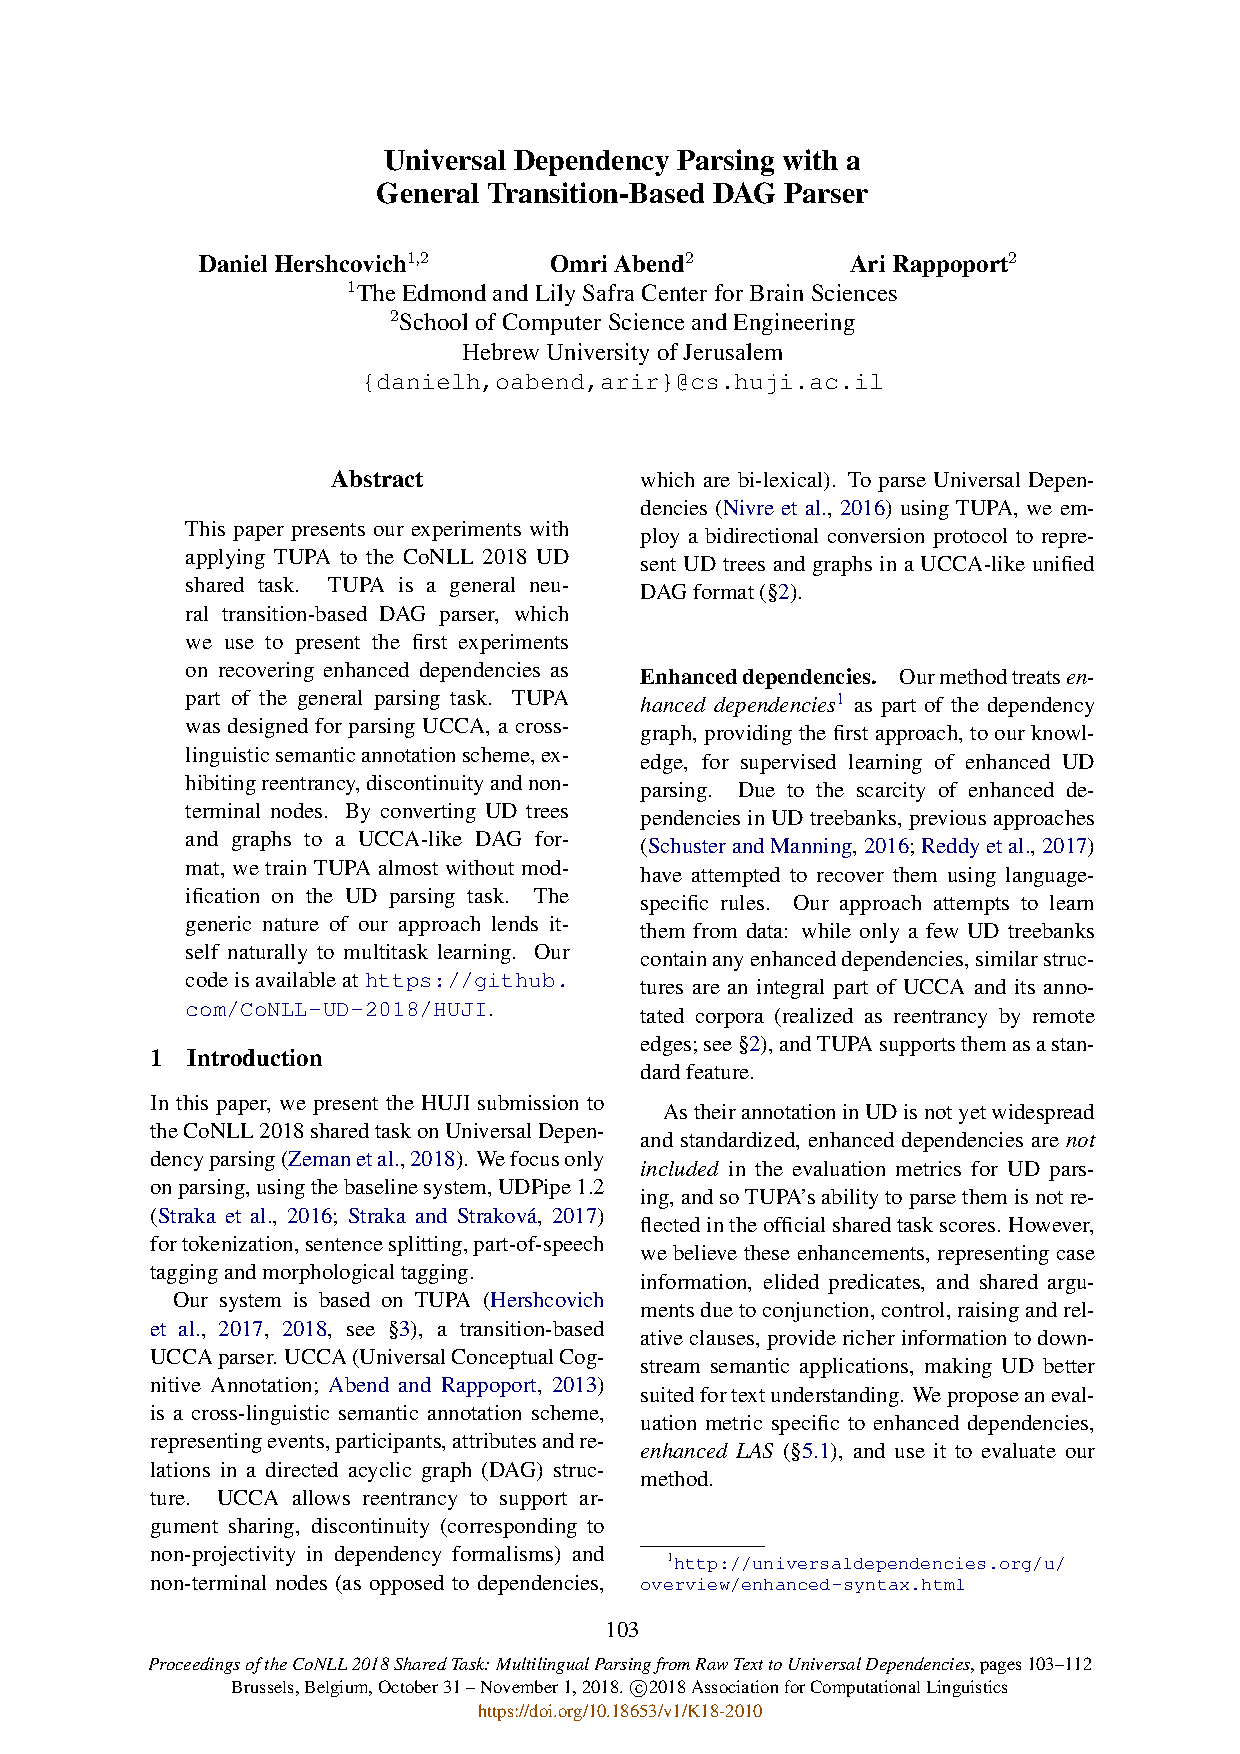
\includepdf[pages=-]{K18-2010.pdf}

\chapter{Content Differences in Syntactic and Semantic Representations \\ (Under Submission)}

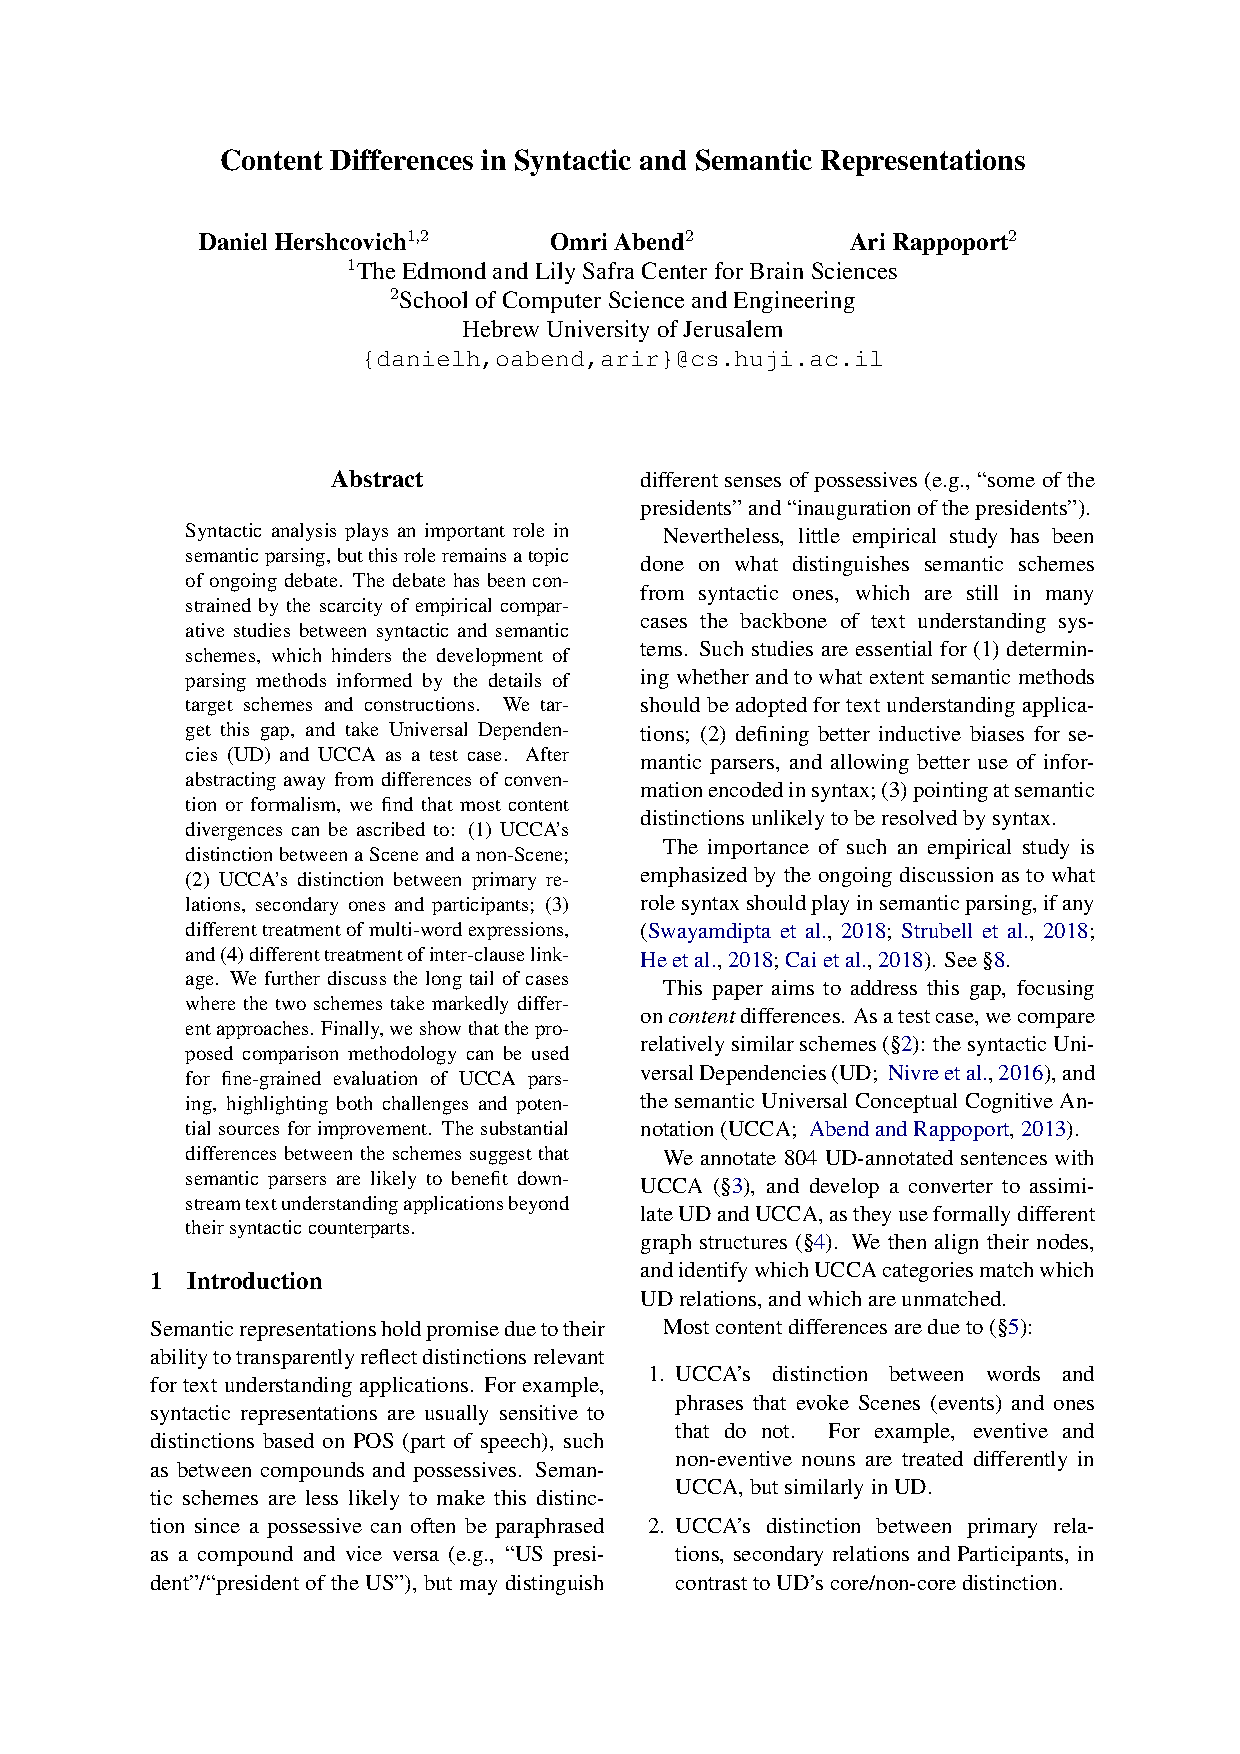
\includepdf[pages=-]{divergences.pdf}

\chapter{Discussion}

Task similarity is an important factor in multitask learning
\citep{E17-2026,E17-1005}.
Empirical comparison with UD reveals that most content differences between it and UCCA are due to:
  \begin{enumerate}
      \item UCCA's distinction of Scene-evoking words and phrases, absent in UD.
      \item UCCA's distinction between primary relations, secondary relations
        and Participants, in contrast to UD's core/non-core distinction.
      \item Different treatment of multi-word expressions (MWEs),
        where UCCA has a stronger tendency to explicitly mark them.
      \item UCCA's conflation of several syntactic realizations of inter-clause linkage,
        and disambiguation of other cases that UD treats similarly.
   \end{enumerate}

  The differences between the schemes are substantial, and suggest that
  UCCA parsing in particular and semantic parsing in general are likely to benefit
  downstream text understanding applications.
  For example, only 73\% of arguments are shared between UCCA and UD,
  i.e., many semantic participants cannot be recovered from UD.

\subsection*{Challenges}

\paragraph{Dataset size.}
Models with a large number of parameters typically require very large
training sets.
Since the UCCA datasets are small in relation to other schemes,
training neural network models on them posed a challenge.
While the data is slowly growing and extended to more languages by further labeling efforts,
multitask learning proved to be an effective method to overcome the data scarcity issue.

\paragraph{Scheme comparison.}
While many distinctions are shared between UCCA and other semantic and syntactic schemes,
they are largely obscured by differences in representation format and convention.
Conversion to a common graph format and assimilation of superficial structures
allowed deep inspection of content divergences and convergences.


\subsection*{Conclusion and Future Prospects}

The research effort to be included in the PhD thesis was completed on December 10, 2018.

UCCA's merits in providing a cross-linguistically applicable,
broad-coverage annotation will support ongoing efforts to incorporate deeper
semantic structures into a variety of applications, such as machine translation
\citep{jones2012semantics} and summarization \citep{liu2015toward}.
The advantage of UCCA as compared to syntactic annotation schemes for machine translation is apparent,
as translation tends to preserve semantic structure more than syntactic structure \citep{sulem2015conceptual}.
Using UCCA as an intermediate representation is thus likely to achieve outputs that are more
semantically similar to the source.

\bibliography{references}
\bibliographystyle{apalike}

\appendix

\chapter{A Transition-Based Directed Acyclic Graph Parser for UCCA \\ Supplementary Notes}

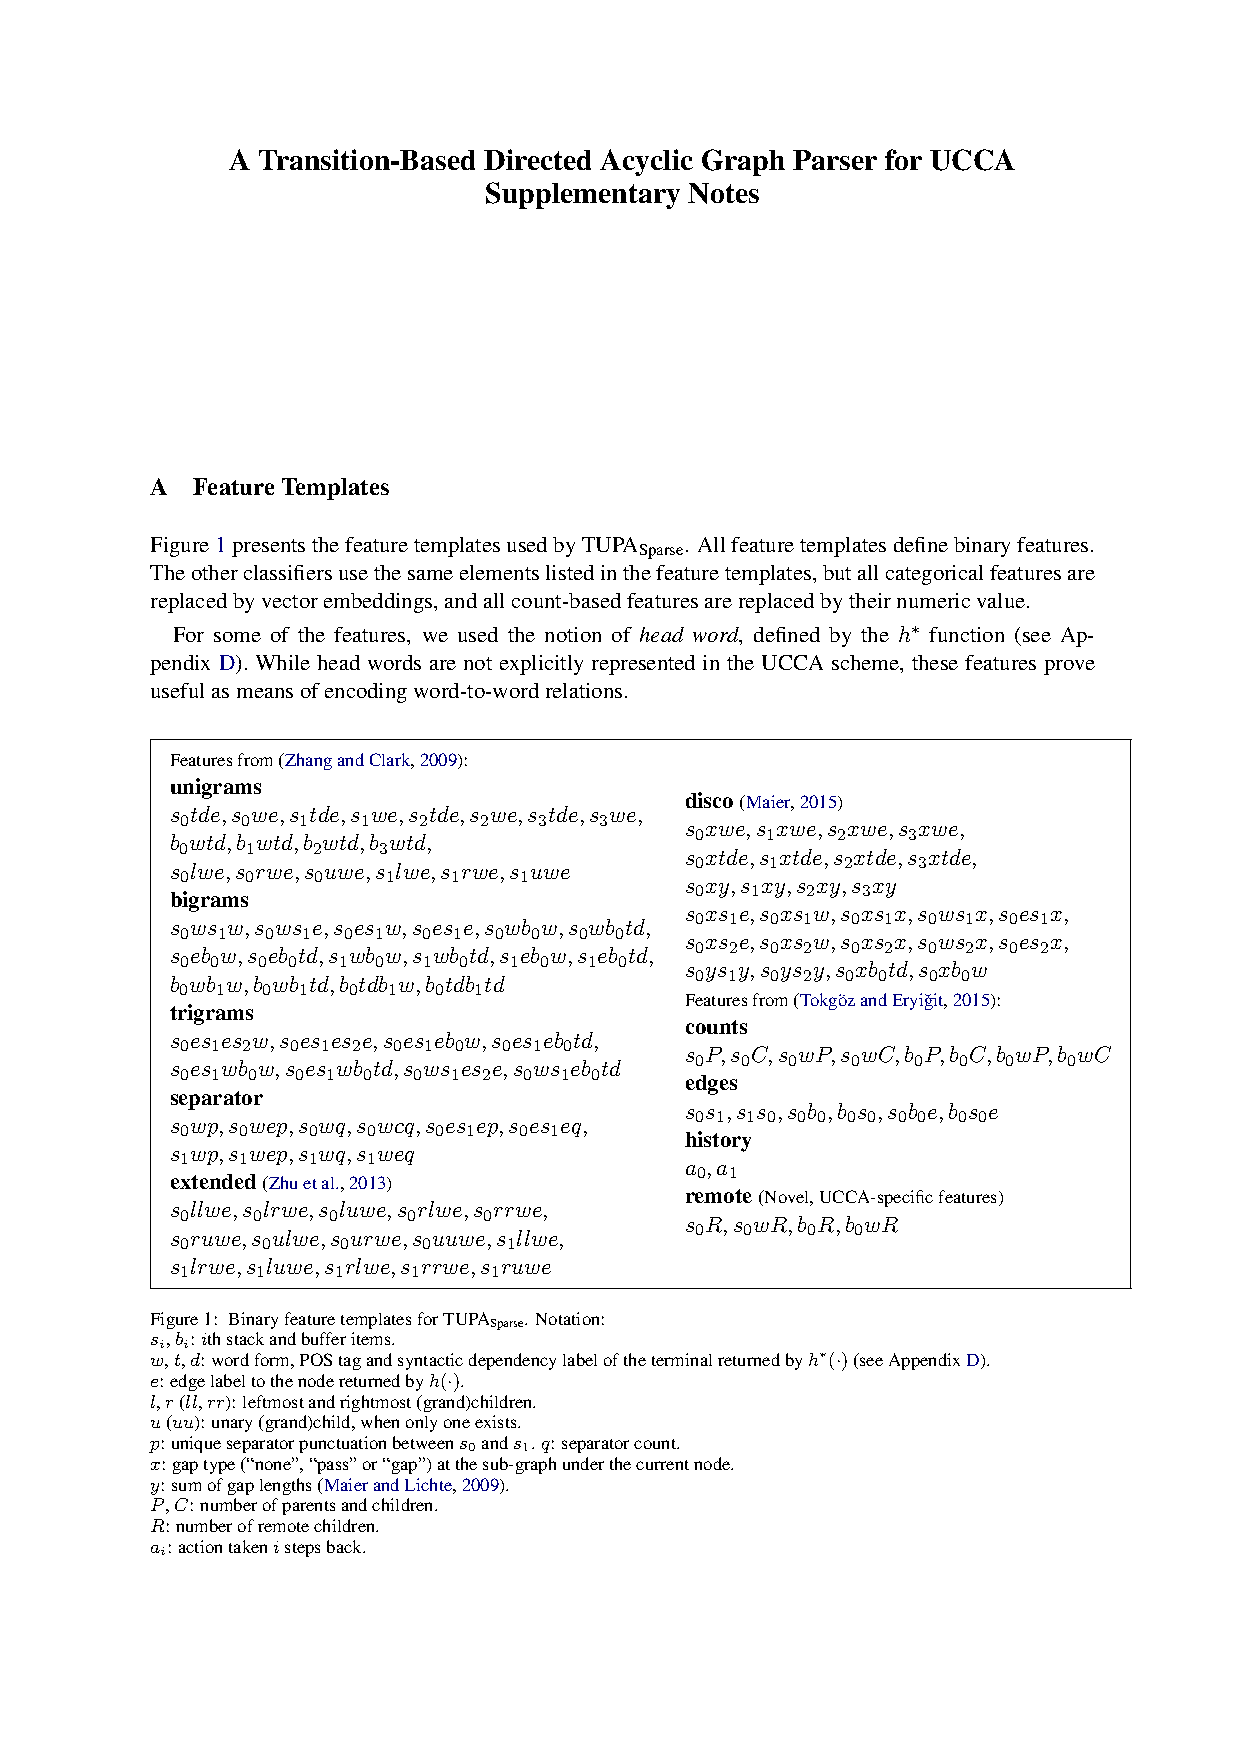
\includepdf[pages=-]{P17-1104_supp.pdf}

\chapter{Multitask Parsing Across Semantic Representations \\ Supplementary Notes}

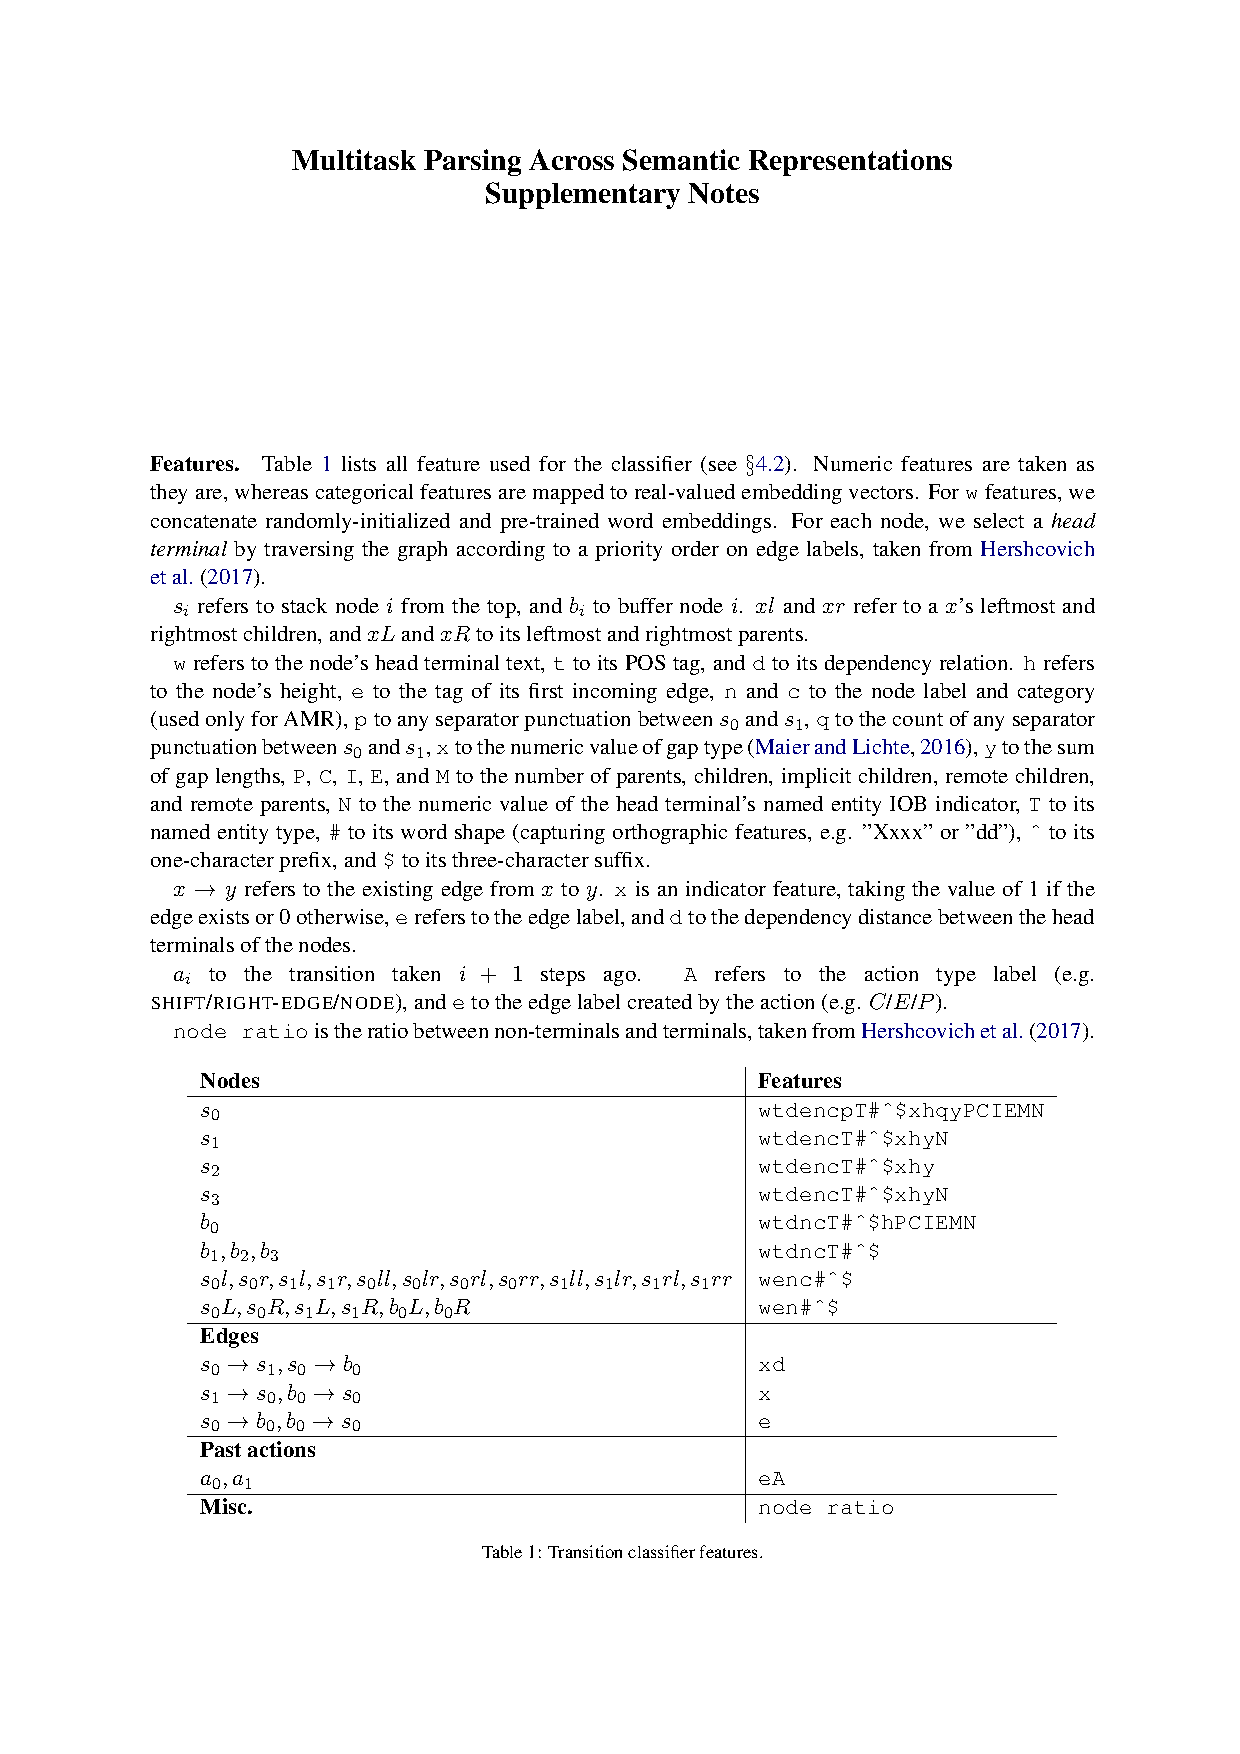
\includepdf[pages=-]{P18-1035_supp.pdf}

\chapter{Content Differences in Syntactic and Semantic Representation \\ Supplementary Notes}

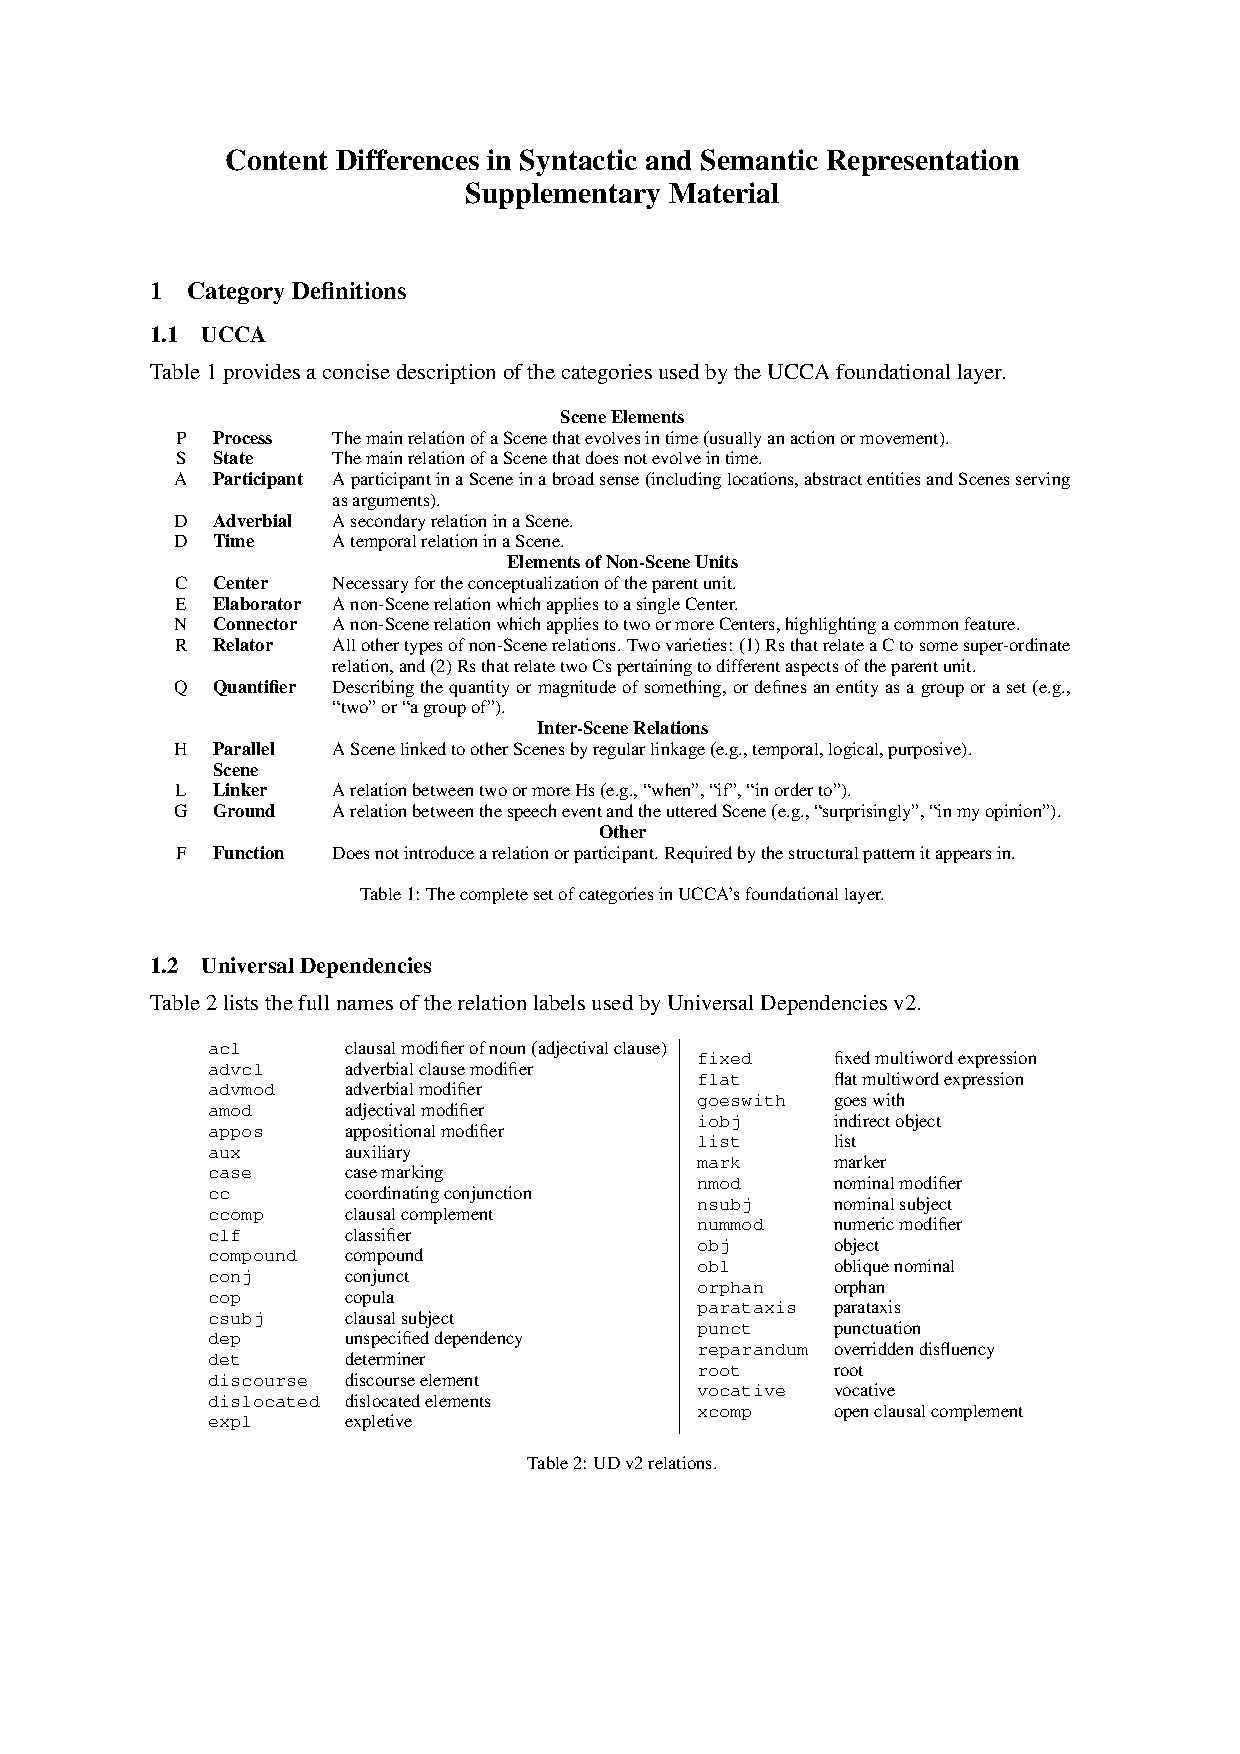
\includepdf[pages=-]{divergences_supp.pdf}

\pagebreak

\section*{\flushright{\heb{תקציר}}}

\pagebreak

\clearpage

\title{}
\author{
\heb{עבודה זו נעשתה בהדרכתם של} \\
\heb{פרופ' ארי רפופורט וד"ר עמרי אבנד}}
\date{}

\maketitle
\clearpage

\title{
\textbf{\heb{ניתוח סמנטי אוניברסלי באמצעות רשתות נוירונים}} \\
\vspace{2cm}
{\large\heb{חיבור לשם קבלת תואר דוקטור לפילוסופיה}}
}
\author{
\heb{מאת}\\
\heb{דניאל הרשקוביץ}
\vspace{2cm}
}
\date{
\heb{הוגש לסנט האוניברסיטה העברית בירושלים} \\
\heb{פברואר 9102}
}

\maketitle
\maketitle

\end{document}
